\documentclass[]{article}

\usepackage[italian]{babel}
\usepackage[margin=20mm, footskip = 20pt]{geometry}
\usepackage{array}
\usepackage{tabularx}
\usepackage{graphicx}
\usepackage{subfiles}
\usepackage{hyperref}
\usepackage{nameref}
\usepackage{titlesec}
\usepackage{longtable}
\usepackage[table]{xcolor}
\usepackage{titling}
\usepackage{lastpage}
\usepackage{ifthen}
\usepackage{calc}
\usepackage{soulutf8}
\usepackage{contour}
\usepackage{float}
\usepackage{fancyhdr}
\usepackage{multirow}
\usepackage{pgfgantt}
\usepackage{lscape}

\newcommand{\hr}{\par\vspace{-.1\ht\strutbox}\noindent\hrulefill\par}

\graphicspath{ {./}
	{./commons/res}
}

%--------------------------------------------------
% Comandi per inserire contenuto del documento
%--------------------------------------------------
\makeatletter

\newcommand\appendToGraphicsPath[1]{%
	\g@addto@macro\Ginput@path{{#1}}%
}

\newcommand{\setTitle}[1]{%
	\newcommand{\@phTitle}{#1}%
}
\newcommand{\phTitle}{\@phTitle}

\newcommand{\setDate}[1]{%
	\newcommand{\@phDate}{#1}%
}
\newcommand{\phDate}{\@phDate}

\newcommand{\setUso}[1]{%
	\newcommand{\@uso}{#1}%
}
\newcommand{\uso}{\@uso}

\newcommand{\setVersione}[1]{%
	\newcommand{\@versione}{#1}%
}
\newcommand{\versione}{\@versione}

\newcommand{\disabilitaVersione}{%
	\renewcommand{\setVersione}[1]{}%
	\renewcommand{\versione}{DISABILITATA}
}

\newcommand{\setResponsabile}[1]{%
	\newcommand{\@responsabile}{#1}%
}
\newcommand{\responsabile}{\@responsabile}

\newcommand{\setRedattori}[1]{%
	\newcommand{\@redattori}{#1}%
}
\newcommand{\redattori}{\@redattori}

\newcommand{\setVerificatori}[1]{%
	\newcommand{\@verificatori}{#1}%
}
\newcommand{\verificatori}{\@verificatori}

\newcommand{\setModifiche}[1]{%
	\newcommand{\@modifiche}{#1}%
}
\newcommand{\modifiche}{\@modifiche}

\makeatother 

%--------------------------------------------------
% Comandi per i documenti esterni e il glossario
%--------------------------------------------------

\newcommand{\dext}[1]{\textsc{#1\textsubscript{\textit{D}}}}

\newcommand{\glock}[1]{\textsc{#1\textsubscript{\textit{G}}}}

%--------------------------------------------------
% Comandi per impostare sottotitoli di quarto e quinto livello
%--------------------------------------------------

\setcounter{secnumdepth}{4}
\setcounter{tocdepth}{4}

\titleformat{\paragraph}
{\normalfont\normalsize\bfseries}{\theparagraph}{1em}{}
\titlespacing*{\paragraph}{0pt}{2.25ex plus 1ex minus .2ex}{1.5ex plus .2ex}

\titleformat{\subparagraph}
{\normalfont\normalsize\bfseries}{\thesubparagraph}{1em}{}
\titlespacing*{\subparagraph}{0pt}{1.75ex plus 1ex minus .2ex}{.75ex plus .1ex}

\appendToGraphicsPath{../../../commons/res/}

%------------------------------
%
% COMANDI DI CONFIGURAZIONE
%
%------------------------------

\setTitle{Verbale esterno \#8}

\setVersione{0.1.0}

\setDate{29-07-2021}

\setResponsabile{}

\setRedattori{Lucia Fenu}

\setVerificatori{Paolo Scanferlato}

\setUso{Esterno}

\setModifiche{
	1.0.0 &   & Responsabile &   & Approvazione \\
	0.1.0 & Lucia Fenu,          Paolo Scanferlato & Amministratore, Verificatore & 04-08-2021 & Stesura iniziale e Verifica}

\begin{document}

	% Direttive per la creazione del titolo tramite comando maketitle
\title{\huge \textsc{\phTitle{}} \\
	\vspace{11pt} \large \textsc{\phDate{}}}

\author{} % Non toccare
\date{} % Non toccare

%--------------------
% Frontespizio
%--------------------

% Logo del gruppo
\begin{figure}[t!]
	\centering
	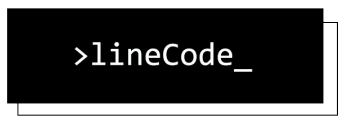
\includegraphics[width=20em]{lclong}
\end{figure}

% Titolo / Nome
\maketitle
\thispagestyle{empty}

% Dati specifici sul doc in forma tabulare
\begin{table}[ht]
	\begin{center}
		\label{tab:Dati sul documento}
		\begin{tabular}{r|l}
			\multicolumn{2}{c}{ \textsc{Dati sul documento} } \\
			\hline
			\textbf{Versione} & \versione{} \\
			\textbf{Uso} & \uso{}  \\
			\textbf{Redattori} & \redattori{} \\
			\textbf{Verificatori} & \verificatori{} \\
			\textbf{Responsabile} & \responsabile{} \\
			\textbf{Destinatari} & lineCode \\
								& prof.\ Vardanega Tullio \\		
								& prof.\ Cardin Riccardo \\
			\ifthenelse{\equal{\uso}{Esterno}}{
								& Sanmarco Informatica
			}{} \\
		\end{tabular}
	\end{center}
\end{table}

\newpage

\renewcommand{\arraystretch}{2} % allarga le righe con dello spazio sotto e sopra
\begin{longtable}[H]{>{\centering\bfseries}m{2cm} >{\centering}m{3.5cm} >{\centering}m{2.5cm} >{\centering}m{3cm} >{\centering\arraybackslash}m{5cm}}
	\rowcolor{lightgray}
	{\textbf{Versione}} & {\textbf{Nominativo}} & {\textbf{Ruolo}} & {\textbf{Data}} & {\textbf{Descrizione}}  \\
	\endfirsthead%
	\rowcolor{lightgray}
	{\textbf{Versione}} & {\textbf{Nominativo}}  & {\textbf{Ruolo}} & {\textbf{Data}} & {\textbf{Descrizione}}  \\
	\endhead%
	\modifiche{}%
\end{longtable}

	\newpage

	%--------------------------------
	%
	% IL CONTENUTO INIZIA DA QUI
	%
	%--------------------------------

	\section{Introduzione}
	\subsection{Luogo e data dell'incontro}
	\begin{itemize}
		\item \textbf{Modalità}: Telematica;
		\item \textbf{Software utilizzato}: Google Meet;
		\item \textbf{Data}: 29 Luglio 2021;
		\item \textbf{Ora di inizio}: 10:00;
		\item \textbf{Ora di fine}: 10:20.
	\end{itemize}

	\subsection{Presenze}
	\begin{itemize}
		\item \textbf{Presenti}:
		\begin{itemize}
			\item Matteo Alba
			\item Giacomo Bulbarelli
			\item Alessandro Chimetto
			\item Alessandro Dindinelli
			\item Lucia Fenu
			\item Paolo Scanferlato
			\item Valton Tahiraj

		\end{itemize}
		\item \textbf{Assenti}:
		\begin{itemize}
			\item Nessuno

		\end{itemize}
		\item \textbf{Partecipanti esterni}:
		\begin{itemize}
			\item Alex Beggiato (referente, Sanmarco Informatica)
		\end{itemize}
	\end{itemize}

	\subsection{Ordine del giorno}
	\begin{enumerate}
		\item Presentazione del lavoro svolto;
		\item Varie ed eventuali
	\end{enumerate}
	\newpage
	\section{Svolgimento}


	\subsection{Presentazione del lavoro svolto}
	Dopo un breve excursus di come il gruppo si è organizzato nel periodo postumo l'accettazione dell'architettura, è stata mostrata al committente una demo del lavoro fino ad ora svolto.\\
	Durante la demo è stato messo in evidenza quali ancora fossero i requisiti mancanti da implementare come:
	\begin{itemize}
		\item Gestione degli ostacoli e dunque la gestione delle collisioni tra più unità presenti;
		\item Inserimento della mappa da file in fase di sviluppo.
	\end{itemize} 
	
	\subsection{Varie ed eventuali}
	Il committente è soddisfatto del lavoro presentato ed ha proposto:
	\begin{itemize}
		\item Nella sezione amministratore in cui si inserisce un nuovo utente, nascondere la password;
		\item durante la presentazione finale del progetto, mostrare una mappa più complessa ad esempio una mappa rettangolare e/o realistica al contesto del ristorante.
	\end{itemize}
	

	\newpage

	\section{Tabella delle decisioni}

	\begin{table} [h!]
		\rowcolors{2}{gray!25}{gray!6}
		\begin{center}
			\begin{tabular} { m{2cm} m{14cm} }
				\rowcolor{lightgray}
				\textbf{ID} & \textbf{Decisione}\\
				VE\_2021-07-29\_8.1 & Nella sezione "inserimento utenti" dell'amministratore, nascondere la password; \\
				VE\_2021-07-29\_8.1& Creare una mappa realistica al contesto\\
			\end{tabular}
		\end{center}
	\end{table}
\end{document}

